\section{Introduction}
Mountain freight corridors expose heavy-duty platoons to a coupled failure mechanism. Sustained downhill braking heats the service brakes and reduces their usable force, while a leader disturbance can increase collision-avoidance demand before pneumatic and auxiliary actuators respond. A thermally constrained truck can therefore become the fleet bottleneck even when its nominal tracking controller remains well behaved. Figure~\ref{fig:framework} summarizes how the physical conflict defines the two-command hard set and current certificate, how predictive and delayed certificates inform four-mode supervision, and how a changed action is reverified before execution; its lower strip is training-only.

Cooperative adaptive cruise control addresses disturbance attenuation \cite{naus2010string,ploeg2011cacc}; brake-fade-aware platoon control addresses thermal degradation \cite{devika2022fade}; and control barrier function (CBF) quadratic programs (QPs) filter unsafe commands \cite{ames2017cbf,xiao2022hocbf}. These strands do not by themselves give an exact, compact test for the joint feasibility of collision demand, thermal/fade restrictions, and auxiliary-brake limits in a heterogeneous truck platoon. The distinctive object here is this physical command geometry, not a generic CBF, multi-agent learning, or differentiable optimization construction.

The hard QP has exactly two decision variables, friction command $u_i^f$ and auxiliary command $u_i^a$. Jerk is a post-action comfort metric, not a slack or decision variable. The certificate depends on the hard set rather than the nominal command, which may be supplied by a learned policy, model-predictive controller, or cooperative cruise controller.

The contributions are:
\begin{itemize}
\item \emph{Exact physical feasibility geometry:} intersect thermal/fade and actuator command intervals with a coupled collision-demand row, and construct $\rho_i$ such that $\rho_i\ge0$ if and only if the declared two-dimensional hard command set is nonempty. This exact sign result includes the low-speed state gate.
\item \emph{Predictive feasibility formulation and distributed monitoring:} define the one-sided $\rho_{i,k}^{H,{\rm cert}}$ under a sound interval-tube assumption, then aggregate the evaluated numerical monitor through an age-aware recursive bottleneck $\rho_{i,k}^{H,{\rm up}}$ with limiting vehicle, horizon, and normalized physical component. The current floating-point monitor is not a verified enclosure of the theoretical certificate.
\item \emph{Certificate-aware dual-brake supervision:} use these quantities to coordinate anticipatory friction/auxiliary allocation, backup, recovery, and upstream requests. Targeted boundary and same-plant comparisons separate command-domain expansion from closed-loop performance.
\end{itemize}

The finite-horizon and distributed constructions carry distinct meanings: a negative numerical predictive value does not prove true future infeasibility, and a delayed upstream minimum is not the instantaneous centralized minimum. Section~VII tests these distinctions. Differentiation through the QP is reported only as a secondary regularity diagnostic.

\begin{figure*}[t]
\centering
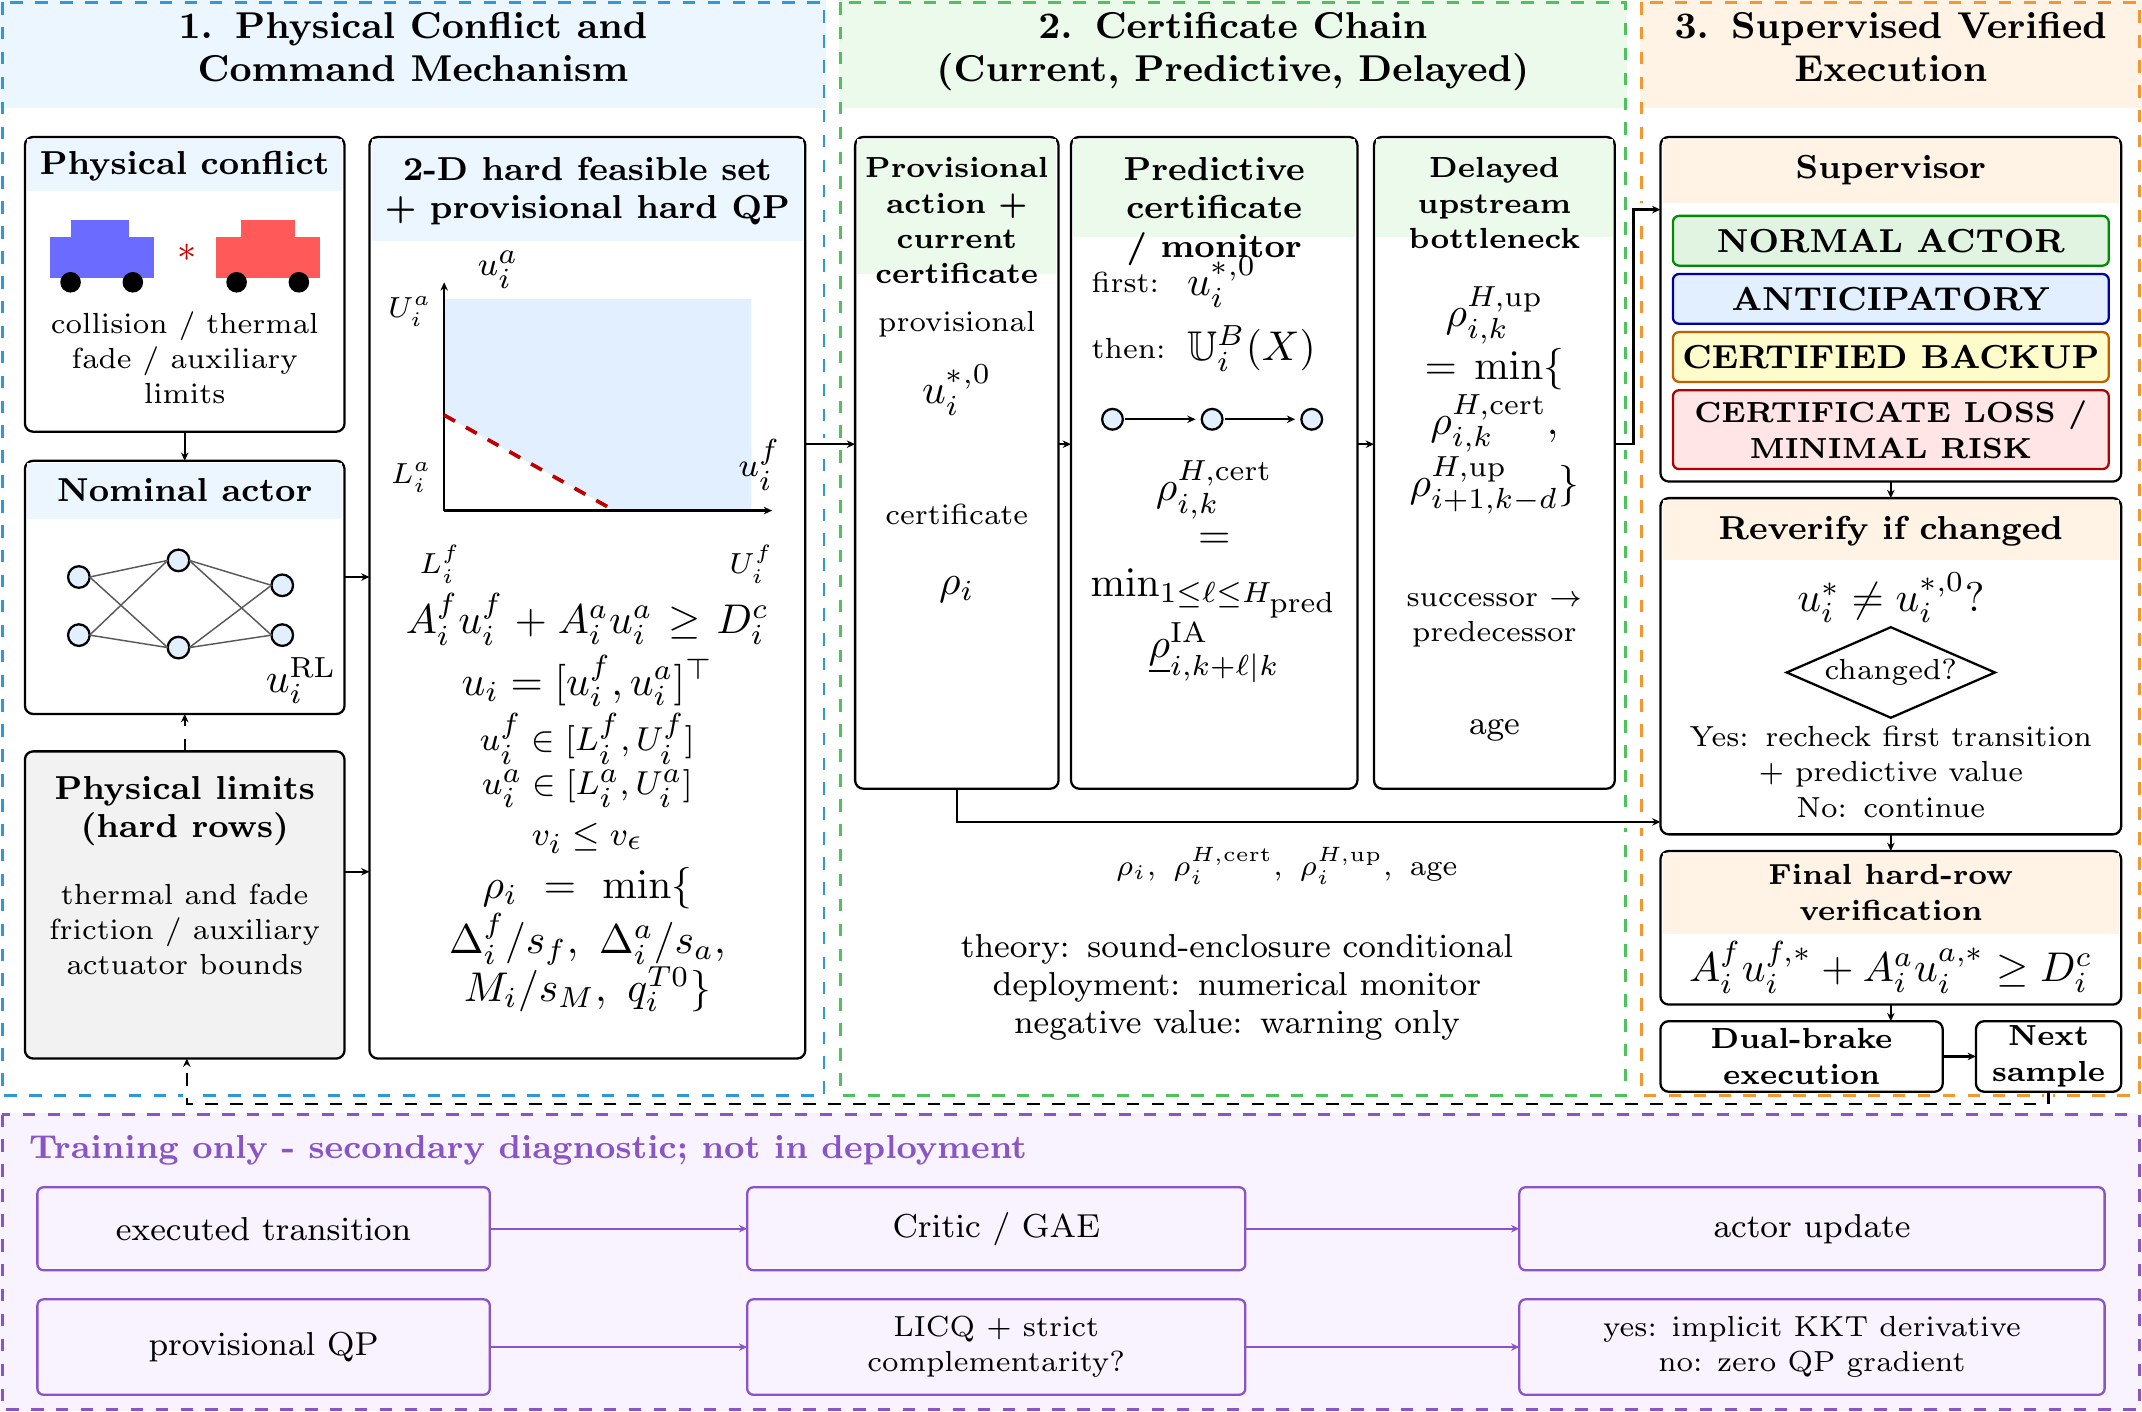
\includegraphics[width=\textwidth]{figures/fig1_desktop66_final.png}
\caption{Certificate-aware dual-brake command mechanism. Collision demand and physical limits define the two-dimensional hard set and instantaneous reserve. The theoretical predictive certificate is conditional on sound enclosure, whereas deployment uses a numerical monitor whose negative value is a warning only. The delayed upstream bottleneck carries age into four-mode supervision. A changed action is reverified before final hard-row verification and execution. The lower strip denotes training-only diagnostics.}
\label{fig:framework}
\end{figure*}
